\section{Ruin Theory for L\'evy Processes}
\begin{defn}
A L\'evy process $X = \{ X(t) \}_{t \in \R^+ }$ is a stochastic process taking values in $\R$ such that $X$ has
\enumb
\item independent increments: $X(t)-X(s)$ is independent of $\{ X(u) : u \leq s \}$ for any ${s<t}$,
\item stationary increments: $X(s+t)-X(s)$ has the same distribution as $X(t)-X(0)$ for any ${s,t>0}$,
\item continuity in probability: $ X(s) \rightarrow X(t) $ in probability as $s \rightarrow t$.
\enume
\end{defn}

\begin{rmk}
Let $X(t)$ be a Levy process. Then
\begin{align*}
\mbbE_0 [e^{sX(t)}] = e^{t\kappa(s)}
\label{LevyExp}
\end{align*}
for a function $\kappa(s)$ called the Levy exponent of $X(t)$.
\end{rmk}
\begin{rmk}[Levy-Khintchine representation of a Levy process]
Let $X(t)$ be a Levy process. Then
\begin{align*}
\kappa(s) = ps + \frac{\sigma^2}{2} s^2 + \int_0^{\infty} [e^{-sy}-1 +sy ] \nu(dy)
\end{align*}
where $p=\mbbE_0[X(1)]$, $\sigma \geq 0$ and $\nu$ is the Levy measure of $-X$, which must satisfy
 $ \int_{0}^{\infty} (y\wedge y^2) \nu(dy) < \infty$.
\end{rmk}
We further note that we will be using the notation $\mbbE_x [X(t)] := \mbbE [X(t) | X(0)=x]$, and in this article we mostly consider cases where the perturbation parameter $\sigma=0$.

In the ruin problem, one assumes
\enumb
\item an initial capital $u>0$,
\item a constant stream of `money' $c>0$ per unit time, and
\item a varying stream of losses represented by a spectrally positive L\'evy process $S(t)$ (i.e. without negative jumps).
\enume
Overall  one observes the behaviour of the process
\[ X(t) = u + ct - S(t), \]
which is also L\'evy, but spectrally negative, that is its jumps represented  can only be negative.

Now, in particular if we assume $S(t) = \sum_{i=1}^{N_{\lambda}(t)} C_i$, i.e. $S(t)$ is a Poisson sum of random variables $C_i$ having the same distribution function $F$ (with the number of $C_i$'s being summed, $N_{\lambda}(t)$, being assumed to be an independent random variable having a Poisson distribution with parameter $\lambda$), we get the Cramer-Lundberg process.
\begin{figure}
\caption{A sample path of a Cram\'er-Lundberg process}
\begin{center}
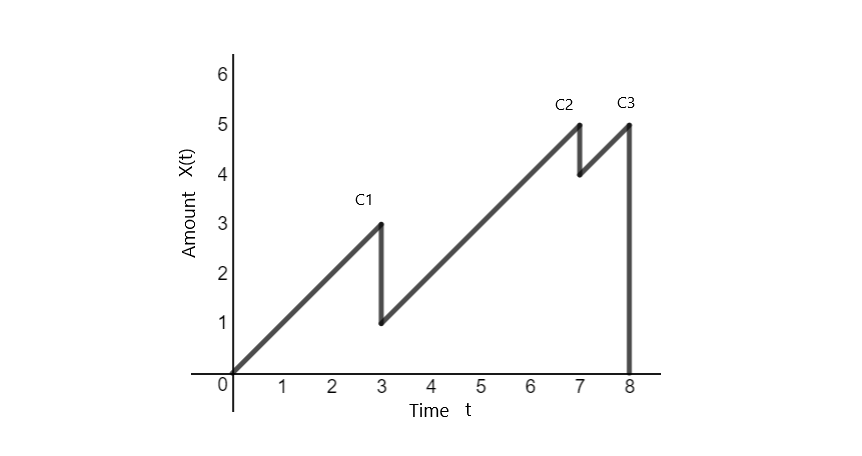
\includegraphics [width=3.3in]{CL1-1.png}
\end{center}
\end{figure}

We define the first passage times
\[ \tau_b^+ = \inf\{ t \geq 0, X(t) > b\}\]
\[ \tau_b^- = \inf\{ t \geq 0, X(t) < b\}\]
as the infimum values at which the process $X(t)$ goes above or below a certain value $b$.\\
Using this notation, we can denote the time of ruin as $\tau = \tau_0^-$. Moreover, if $X(t) > 0$ $\forall t\geq 0$, then we say $\tau = + \infty$.

Let $t, u >0$. The probability of ruin before time $t$ and given initial value $u$ is written as
\[\Psi(t|u) = \mathbb{P} [\tau < t | X(0)=u ].  \]
We refer to this scenario ruin in finite time.\\

Alternatively, one can study probabilities of survival in finite time by observing the function
\[ \bar {\Psi} (t|u) = \mathbb{P} [\tau \geq t | X(0)=u ] = 1 - \Psi (t|u) . \]

Letting the value of $t$ approach infinity, we get a quantity which can be interpreted as the probability of eventual ruin, or ruin in infinite time.

Let $u >0$. The probability of ruin given initial value $u$ is written as
\[\Psi(u) = \mathbb{P} [\tau < +\infty | X(0)=u ]. \]
Same as in the last definition, we also can study
\[ \bar {\Psi} (u) = \mathbb{P} [\tau = + \infty | X(0)=u ] = 1 - \Psi (u). \]

The \rp \ is a measure of the risk associated to a financial company.

For the case Cramer-Lundberg case, the following formula which may be inferred form the work of Pollaczek, Khinchine (\cite{Rolski}) was found great of great use in ruin theory (and in queueing theory) :
\[\hat \Psi(s) = \int_0^{\infty} e^{-s u} \Psi(u) du
= \frac{\lambda (m_1 - \hat{\bar{F}}(s))}{s (c-\lambda \hat{\bar{F}}(s)) }\]
where $\hat \Psi(s)$ and $\hat{\bar{F}}(s)$ are the Laplace transforms of the ruin function and the survival function of the claim distributions respectively, and $m_1$ is the first moment of the claims, which will be assumed from now on to be finite.

We state now several forms of this result,  emphasizing the relationship of $\hat \Psi(s)$ to the  crucial  Levy exponent $\kappa (s)$ of the underlying process. This is important, since results expressed in terms of $\kappa (s)$ hold typically for all \sn \lev \procs.

\begin{thm}[The Pollaczek-Khinchine formulas for the ruin function Laplace transform]
Let $X(t) = u + ct - S(t), \quad S(t) = \sum_{i=1}^{N_\lambda (t)} C_i$ be a Cram\'er Lundberg risk process and $\Psi$ its corresponding ruin function. Then the Laplace transforms of the ruin function and its corresponding survival function can be expressed as
\begin{align*}
\hat \Rui(s) &= \int_0^{\infty} e^{-s u} \Rui(u) du
= \frac{\lambda (m_1 - \hat{\bar{F}}(s))}{s (c-\lambda \hat{\bar{F}}(s)) } = \frac{1}{s}- \frac{ \kappa'(0)}{ \kappa(s)} \\
\hat \sRui(s) &= \int_0^{\infty} e^{-s u} \sRui(u) du = \frac{1}{s} - \hat \Rui(s) = \frac{\kappa'(0)}{\kappa(s)}.
\end{align*}
It is also possible to express this result in terms of 
the equilibrium density $f_e(x):=\bar{F}(x)/m_1$ and of $\rho =(\lambda m_1)/c$, since for Cramer Lundberg processes $\kappa(s) =  cs( 1- \rho \hat f_e(s)) $.
\end{thm}